\documentclass{standalone}

%\usepackage[top=15mm, bottom=15mm, left=15mm, right=15mm]{geometry}
\usepackage{tikz}

\usetikzlibrary{calendar}

\begin{document}

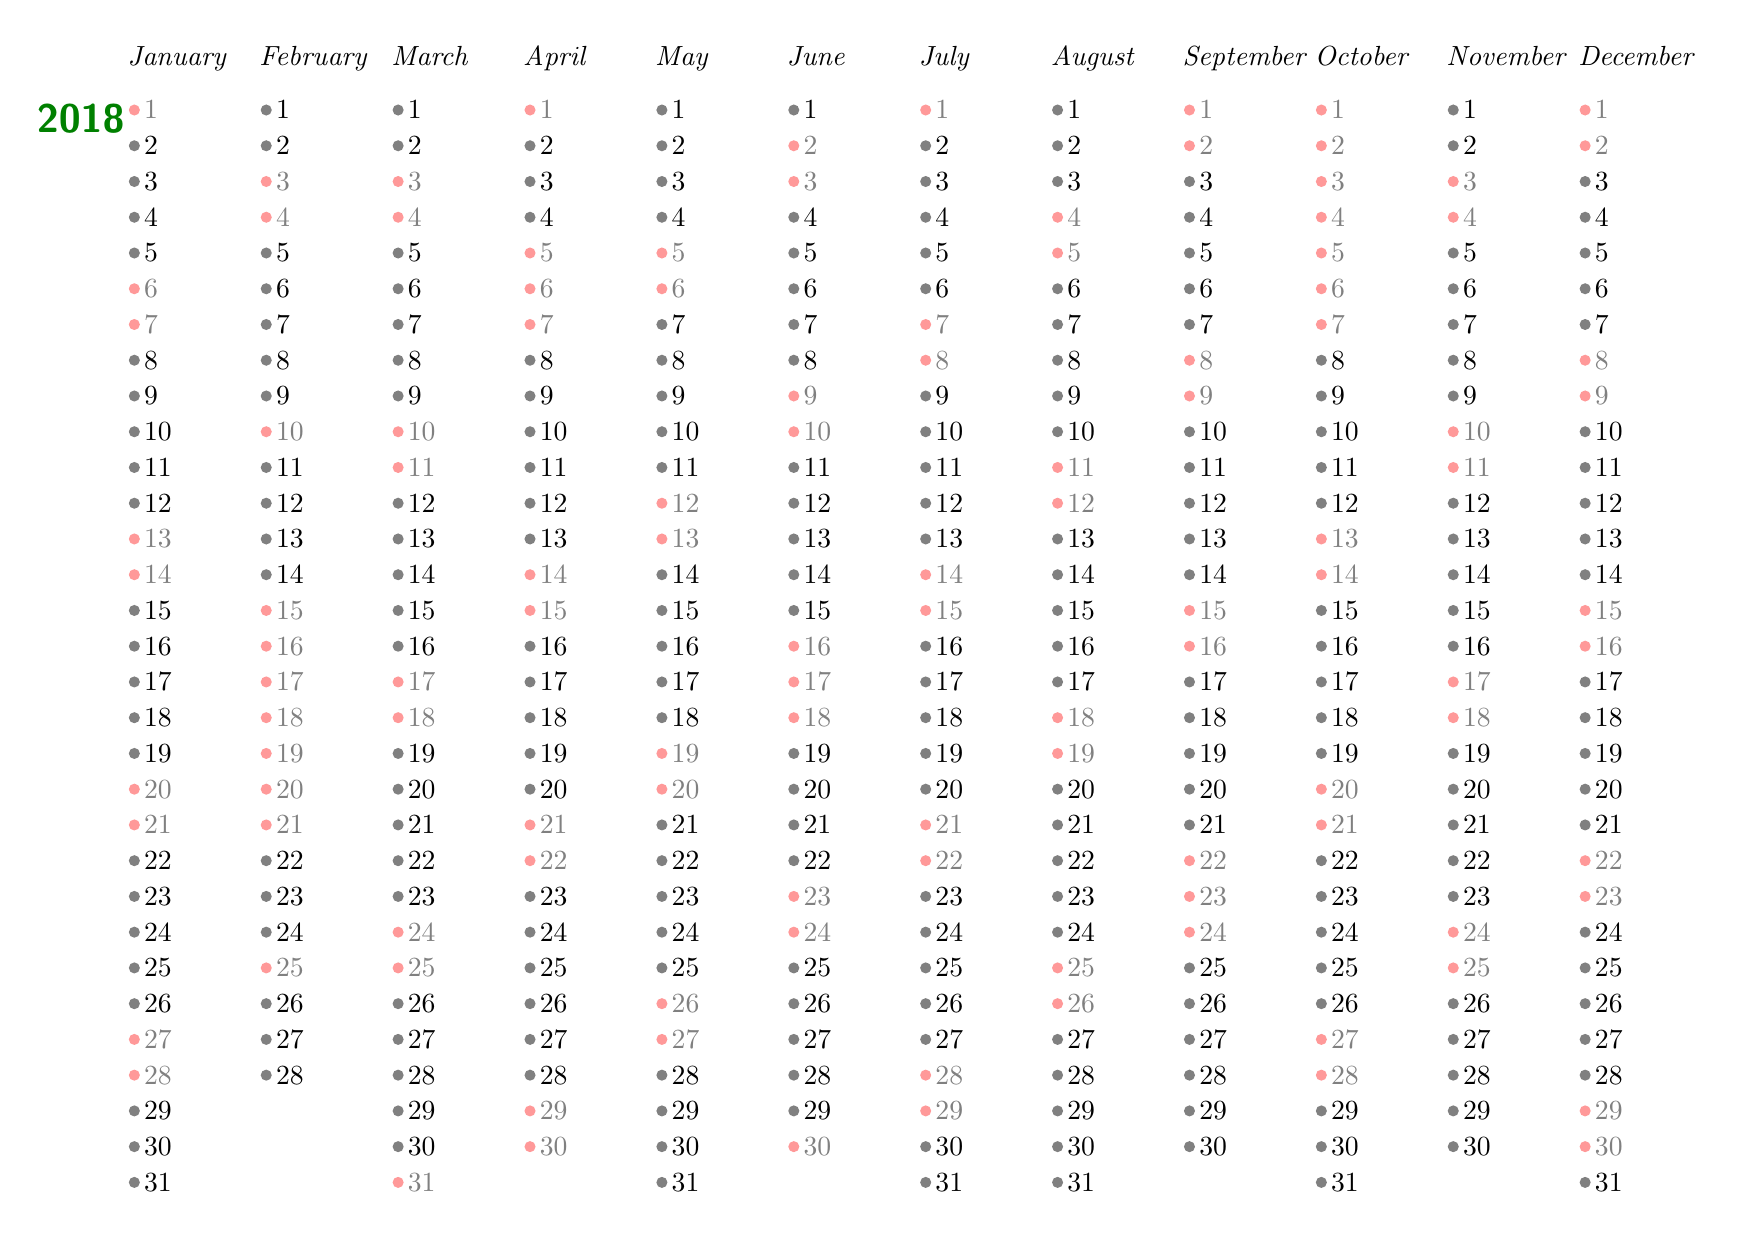
\begin{tikzpicture}[every calendar/.style={
		 day code = {\ifdate{equals=2018-01-01, between=2018-02-15 and 2018-02-21, between=2018-04-05 and 2018-04-07, between=2018-04-29 and 2018-04-30, between=2018-06-16 and 2018-06-18, between=2018-09-22 and 2018-09-24, between=2018-10-01 and 2018-10-07} %Rest weekday
		             {\fill[red!40] (-8pt, 0) circle[radius=2pt] node[name=\pgfcalendarsuggestedname,every day,right, black!50]{\tikzdaytext};}
		             {\ifdate{equals=2018-02-11, equals=2018-02-24, equals=2018-04-08, equals=2018-04-28, between=2018-09-29 and 2018-09-30} %Non-rest weekend
		                 {\fill[black!50] (-8pt, 0) circle[radius=2pt] node[name=\pgfcalendarsuggestedname,every day,right, black]{\tikzdaytext};}
		                 {\ifdate{equals=2017-01-02} %Half-rest day
		                     {\draw[red!50] (-8pt, 0) circle[radius=2pt] circle[radius=1pt, fill=red!50] node[name=\pgfcalendarsuggestedname,every day,right, black]{\tikzdaytext};}
		                     {\ifdate{weekend} %Weekend
		                         {\fill[red!40] (-8pt, 0) circle[radius=2pt] node[name=\pgfcalendarsuggestedname,every day,right, black!50]{\tikzdaytext};}
		                         {\fill[black!50] (-8pt, 0) circle[radius=2pt] node[name=\pgfcalendarsuggestedname,every day,right, black]{\tikzdaytext};}
                                }
                            }
		             }
                       },
            month label above left,
            month text={\textit{\%mt}},
            every year/.append style={font=\Large\sffamily\bfseries,
                green!50!black},
		 day list downward, 
        }]

\matrix[column sep=1em, row sep=1em, text width=25pt] {
    \calendar [dates=2018-01-01 to 2018-01-last, name=cal01];&
    \calendar [dates=2018-02-01 to 2018-02-last, name=cal02];&
    \calendar [dates=2018-03-01 to 2018-03-last, name=cal03];&
    \calendar [dates=2018-04-01 to 2018-04-last, name=cal04];&
    \calendar [dates=2018-05-01 to 2018-05-last, name=cal05];&
    \calendar [dates=2018-06-01 to 2018-06-last, name=cal06];&
    \calendar [dates=2018-07-01 to 2018-07-last, name=cal07];&
    \calendar [dates=2018-08-01 to 2018-08-last, name=cal08];&
    \calendar [dates=2018-09-01 to 2018-09-last, name=cal09];&
    \calendar [dates=2018-10-01 to 2018-10-last, name=cal10];&
    \calendar [dates=2018-11-01 to 2018-11-last, name=cal11];&
    \calendar [dates=2018-12-01 to 2018-12-last, name=cal12];&
    \\
};

\node [anchor=east, green!50!black] at (cal01-2018-01-01.base west) {\Large\sffamily\bfseries{2018}};

\end{tikzpicture}

\end{document}